\documentclass[../memoria.tex]{subfiles}
\begin{document}
\label{fundamentos y discusion bibliografica}

Re-ID se define como la tarea de establecer correspondencia entre imágenes de personas tomadas desde cámaras diferentes. Un sistema típico de Re-ID ejecuta este proceso en dos fases \cite{bedagkar2014survey}: (1) generación de una identificación (descriptor) para cada persona detectada, y (2) comparación entre descriptores, tal como se muestra en la figura \ref{fig:sistemaReID}. 

\begin{figure}[h!]
  \centering
  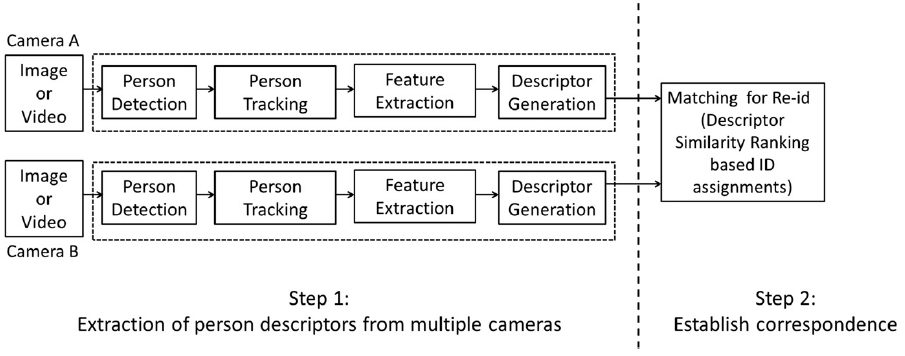
\includegraphics[width=\textwidth]{diagrama1.png}
  \caption{Sistema de Re-ID \cite{bedagkar2014survey}}
  \label{fig:sistemaReID}
\end{figure}

En una primera fase, se genera el descriptor de una persona detectada en múltiples escenas (capturadas con una o varias cámaras). En una segunda fase, se establece la correspondencia entre descriptores, determinando si estos coinciden con la misma persona o son individuos distintos.

La efectividad de un sistema de Re-ID se evalúa mediante una curva CMC (\emph{Cumulative Matching Characteristic}), que mide la probabilidad de que el sistema entregue correctamente el descriptor que corresponde al descriptor consultado, donde la respuesta está compuesta por $k$ candidatos, y es considerada correcta si el descriptor que hace match con la consulta está entre dichos candidatos \cite{decann2012can}. Luego, CMC indica la proporción de respuestas correctas obtenidas para distintos valores de $k$:$${\rm\ Precisi\acute{o}n} = \frac{{\rm \#\ respuestas\ correctas}}{{\rm\ \#\ consultas\ realizadas}}\times 100$$
\todo{aclarar que el denominador corresponde sólo a las predicciones positivas}


Las tareas típicas de la primera fase incluyen \cite{yilmaz2006object}:
\begin{itemize}
	\item \underline{Detección de personas:} se establece la presencia de personas en una escena. Para esto, se pueden utilizar algoritmos de aprendizaje supervisado cuando se cuenta con una base de datos con imágenes etiquetadas \cite{dalal2005histograms}. En el caso de un video, existen varias imágenes consecutivas (cuadros o \emph{frames}), lo que permite detectar cuando la persona se mueve o desplaza por la escena, según los cambios producidos en cada píxel. Esto se conoce como segmentación entre primer y segundo plano (que corresponden al movimiento y regiones estáticas, respectivamente).

	La detección del segundo plano permite eliminar de la imagen todo lo que no forma parte de la persona, ocultando todo el conjunto de píxeles que permanezcan sin cambios. Para esto, se utiliza un mapa de bits, que se superpone a la imagen original, convirtiendo el segundo plano en un mismo valor (bit cero: color negro), dejando los píxeles del primer plano inalterados (bit uno: color original) \cite{bouwmans2008background}. Luego, un algoritmo de detección de bordes \cite{canny1986computational} encuentra fronteras entre regiones similares, obteniendo la silueta del objeto o persona en movimiento. En algunas ocasiones, cuando existe alto grado de contraste entre una persona y el fondo (como en una toma a la misma altura del individuo) la detección de bordes puede prescindir de la segmentación. Sin embargo, ésta permite obtener bordes con menos posibilidad de error, dado que todo el fondo tiene un mismo valor \cite{bouwmans2008background}.

	Uno de los problemas de utilizar segmentación entre primer y segundo plano para detectar personas, es el ruido producido por cambios de iluminación repentinos y otros elementos en movimiento (vehículos, animales, sombras, etc.), lo que hace almacenar regiones de la imagen que no contiene personas, siendo analizadas erróneamente más adelante. Este problema se puede enfrentar utilizando un clasificador binarios sobre imágenes, seleccionando aquellas que sean clasificadas como personas \cite{nakajima2003full}. Una solución propuesta es filtrar las siluetas detectadas con base en su posición y forma (ver capítulo \ref{modelo desarrollado}).

	\item \underline{Seguimiento de la persona:} en esta tarea, se sigue la trayectoria realizada por una persona dentro de un FOV. De esta forma, la Re-ID se utiliza para lograr seguir de personas a través de varias cámaras. Por otro lado, durante el seguimiento individual de cada cámara, se pueden inferir datos de la persona, como: su dirección de movimiento, ubicación inicial y final. Estos datos pueden ser usados para filtrar los candidatos a re-identificar.
	
	\begin{figure}
	  \centering
	  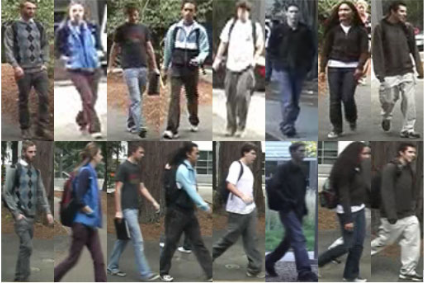
\includegraphics[width=0.5\textwidth]{viper.png}
	  \caption{Ejemplos Data Set VIPeR: cada columna muestra una de las 632 personas.}
	  \label{fig:viper}
	\end{figure}

	\item \underline{Extracción de características:} en esta tarea, se extraen las características que formarán el descriptor de la persona. Las características pueden ser de distintos tipos, entre ellos \cite{vezzani2013people}: 

		\begin{itemize}
			\item \underline{Color:} una imagen está compuesta por píxeles cuyos valores dependen del espacio de colores empleado. Un espacio de colores está compuesto por varios canales, por ejemplo, el espacio RGB está conformado por los canales rojo (R), verde (G) y azul (B); o el espacio HSV, compuesto por los canales de tonalidad (H), saturación (S) y valor (V). El color como característica de apariencia se ha empleado en forma de histogramas \cite{gheissari2006person, gray2008viewpoint, javed2008modeling, oliveira2009people, farenzena2010person, prosser2010person, zheng2011person}. Se pueden utilizar diferentes canales de colores y sus combinaciones. Por ejemplo, del espacio de colores HSV, se ha empleado sólo el tono \cite{oliveira2009people},  tono y saturación \cite{gheissari2006person}, o los tres canales del espacio \cite{farenzena2010person}. Por otro lado, histogramas del espacio de colores RGB fueron utilizados en \cite{prosserxiang2008multi, javed2008modeling, berdugo2010object}. Otros\cite{gray2008viewpoint, prosser2010person, zheng2011person} han adoptado una concatenación de histogramas de los canales de los espacios RGB, YCbCr y HSV (sólo tono y saturación). Un dataset de imágenes (VIPeR) \cite{gray2008viewpoint} ha sido ampliamente utilizado como \emph{benchmark}, debido a la cantidad de personas (632), las que fueron fotografiadas (48x128 píxeles) en ambientes exteriores, siempre desde dos ángulos distintos y en diferentes posiciones (ver figura \ref{fig:viper}). Las pruebas determinan que los canales más discriminantes (en orden descendente) para Re-ID personas, son: tono, saturación, azul, rojo y verde \cite{mazzon2012person}. Por último, pruebas de Re-ID con el dataset VIPeR utilizando descriptores compuestos únicamente por histogramas de colores y comparándolos con distancia euclidiana, para rangos $k=1$ y $k=20$ en la curva CMC, se obtiene un 6\% y 38\% de precisión de reconocimiento, respectivamente \cite{hirzer2012relaxed}.
			
			\item \underline{Forma:} se refiere a datos de la silueta detectada (altura, ancho, ejes de simetría, relación entre ancho y altura, etc.). Se han propuesto algoritmos que hacen uso de la simetría de la figura humana \cite{farenzena2010person}: \emph{Symmetry-Driven Accumulation of Local Features}, SDALF. El método segmenta la silueta de la persona en tres partes: cabeza, torso y piernas (ver figura \ref{fig:sdalf}), comparando cada parte con su homóloga correspondiente. Luego, se buscan ejes verticales de simetría para cada una de las partes mencionadas, con el objetivo de ponderar las features (histogramas del espacio HSV de subregiones de píxeles) en relación a la distancia de éstas con el eje, destacando aquellas features que estén cercanas al eje, dado que tienen menor probabilidad de pertenecer al segundo plano de la imagen. Una evaluación de SDALF con el dataset VIPeR, obtiene para $k=1$ y $k=20$ en la curva CMC, un 20\% y 65\% de precisión de reconocimiento, respectivamente \cite{farenzena2010person}. %Un enfoque similar fue presentado en \cite{park2006vise}, donde se extraen tres histogramas para modelar cabeza, torso y piernas por separado.

			
			\item \underline{Posición:} cuando los FOV entre cámaras están superpuestos, la posición de una persona puede ser utilizada para Re-ID, dado que el movimiento capturado en cada cámara es equivalente \cite{khan2003consistent, calderara2008hecol}.
			\begin{table}
			  \begin{center}
			    \begin{tabular}{cccc}
			      \hline
			      Escena    & personas  & ocurrencias & exactitud \\
			      \hline
			      Salón     & 12        & 80          & 89.3\% \\
			      Corredor  & 58        & 38          & 70.4\% \\
			      \hline
			    \end{tabular}  
			  \end{center}
			  \caption{Resultados obtenidos en  \cite{hu2008people}}
			\label{resultados SIFT hu2008}
			\end{table}

			\item \underline{Textura:} entrega la disposición espacial de los colores de una imagen \cite{stockman2001computervision}. Se ha representado por puntos seleccionados de la imagen (puntos de interés o \emph{keypoints}), cuyas propiedades se mantienen invariables a cambios de tamaño \cite{lowe1999object, bay2006surf}, permitiendo Re-ID objetos capturados a distintas distancias. Generalmente, estos puntos se encuentran en la frontera entre regiones con colores muy distintos. Algunos enfoques buscan Re-ID personas que abandonan y luego reingresan al FOV de una misma cámara, buscando enfrentar de forma robusta, cambios de iluminación, postura y escala \cite{hu2008people}. Para formar el descriptor de cada persona, se emplean histogramas de colores y keypoints seleccionados por un algoritmo típico de transformación de características \cite{lowe1999object} (Scale-invariant feature transform, SIFT). Los keypoints detectados por SIFT corresponden a una región circular de la imagen con una dirección, siendo representada por las coordenadas de su centro $(x,y)$, el tamaño (radio) y dirección (ángulo). El proceso de comparación se realizó con un clasificador binario. Las pruebas se realizaron con videos\footnote{Proyecto CAVIAR IST 2001 37540 financiado por la Comunidad Europea, disponible en \url{http://homepages.inf.ed.ac.uk/rbf/CAVIAR/}} en dos escenarios distintos, donde aparece un grupo limitado de personas que abandonan e ingresan en reiteradas ocasiones, obteniendo una exactitud desde un 70.4\% hasta 89.3\% (ver cuadro \ref{resultados SIFT hu2008}). Un trabajo comparable a \cite{hu2008people} es presentado en \cite{hamdoun2008person}, donde se emplea el mismo dataset y las características son keypoints detectados con SIFT. La precisión de Re-ID obtenida en este trabajo depende de la cantidad mínima de keypoints coincidentes requeridos para establecer a sus respectivos descriptores como un match (ver cuadro \ref{resultados SIFT hamdoun2008person}).

		\end{itemize}
	
	\begin{table}
	  \begin{center}
	    \begin{tabular}{cc}
	      \hline
	      keypoint necesarios & Precisión \\
	      \hline
	      40 & 99\% \\
	      30 & 95\% \\
	      20 & 85\% \\
	      10 & 10\% \\
	      \hline
	    \end{tabular}  
	  \end{center}
	  \caption{Resultados obtenidos en  \cite{hamdoun2008person}}
	\label{resultados SIFT hamdoun2008person}
	\end{table}

	\begin{figure}
	  \centering
	  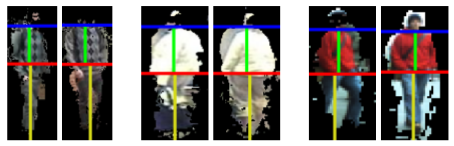
\includegraphics[width=0.6\textwidth]{sdalf.png}
	  \caption{Algoritmo SDALF: Segmentación de la imagen usando ejes horizontales (partes asimétricas) y verticales (partes simétricas).}
	  \label{fig:sdalf}
	\end{figure}

	\item \underline{Generación del descriptores:} en esta tarea, las características detectadas son organizadas en estructuras de datos (ej. vector de $n$ dimensiones), las que reciben el nombre de descriptores. Generalmente se calculan estadísticas sobre las características, para generar una representación sucinta de éstas (ej. histogramas). %Los descriptores generados pueden ser todos de tamaño fijo o variable. Un ejemplo del primer caso son los histogramas, cuya cantidad de dimensiones es independiente del tamaño de la imagen y los colores presentes en ella, dependiendo el tamaño sólo del espacio de colores empleado. Un algoritmo típico de transformación de características \cite{lowe1999object} (Scale-invariant feature transform, SIFT) encuentra keypoints en una imagen, generando descriptores de tamaño variable (cantidad de puntos seleccionados es variable dependiendo de la complejidad de la imagen). Sin embargo, la representación de cada punto es un vector de tamaño fijo: coordenadas $(x,y)$, tamaño, ángulo, responsive y octaba. 
\end{itemize}

La segunda fase de un sistema de Re-ID define la forma de asociar descriptores. Para esto, se determina si un par de descriptores corresponden o no a una misma persona. 

Para encontrar una coincidencia (\emph{match}) se han propuesto varios algoritmos. Uno típico calcula la distancia Euclidiana entre el descriptor consultado (\emph{query}) con todos los posibles candidatos (vecinos) y luego elije a los $k$ candidatos que se encuentren a menor distancia, técnica conocida como el k-ésimo vecino más cercano (k Nearest Neighbor, k-NN). Una mejora utiliza una métrica de distancia que considera patrones estadísticos obtenidos de ejemplos en forma de tuplas ($A,B,etiqueta$), donde $A$ y $B$ son descriptores, y la etiqueta indica si éstos son un match o no \cite{weinberger2009dml, zheng2013reidentification, dikmen2011pedestrian, hirzer2012person, hirzer2012relaxed, zheng2011person}.

Para comparar dos descriptores compuestos por keypoints (ej. SIFT), se calcula la distancia de cada keypoint de un descriptor con todos los keypoints del otro descriptor, estableciendo una correspondencia positiva si existe un par de keypoints a una distancia lo suficientemente pequeña, menor a cierto umbral. Si se cuenta con varias imágenes por persona, se puede utilizar un sistema de votación, el cual asigna un voto al descriptor candidato siempre que éste posea el keypoint más similar (a menor distancia) a un keypoint del descriptor consultado, emitiendo tantos votos como keypoints tenga éste, seleccionando luego al descriptor candidato con más votos \cite{hamdoun2008person}. 

En general, la comparación de descriptores se puede realizar: (a) midiendo su similitud usando métricas de distancia directa, (b) utilizando algoritmos de aprendizaje supervisado o (c) aplicando métodos de optimización \cite{mazzon2012person}.

Las métricas de distancia directas estiman diferencias entre descriptores para determinar la correspondencia. La métrica más usada es la distancia Euclidiana, utilizada sobre descriptores basados en color \cite{farenzena2010person, bak2010person} y puntos de interés \cite{gheissari2006person}. Sin embargo, utilizar únicamente métricas de distancia directa no siempre permite establecer una correcta similitud entre descriptores, pues cuando la mayoría de las features de un descriptor coincide con los de otro correspondiente a una persona desigual, los descriptores respectivos estarán cercanos entre sí. Del mismo modo, para una misma persona que cambia de apariencia (cambio drástico en varios features a causa de diferente iluminación, postura de la persona, punto de vista, etc.), sus respectivos descriptores se encontrarán a mayor distancia. Como consecuencia, al emplear sólo una distancia tradicional, se ignora cualquier regularidad estadística, la que podría ser estimada con algoritmos de aprendizaje supervisados \cite{zheng2011person, prosser2010person}. Un sistema de Re-ID de personas que sólo emplea una métrica directa, no es robusto ante cambios de iluminación, razón por la que se requiere una calibración previa en la red de cámaras \cite{gilbert2006tracking, porikli2003multi, stein1999tracking, javed2008modeling}.

Por otro lado, varias técnicas de aprendizaje automático (Machine Learning, ML) se han empleado en sistemas de Re-ID para distintos objetivos. Por ejemplo, un clasificador binario puede distinguir entre descriptores positivos (match) y negativos (mismatch). Un sistema de Re-ID basado en un clasificador binario, puede etiquetar un par de descriptores como match incluso si éstos presentan más diferencias que otro par compuesto por descriptores de personas distintas \cite{prosser2010person}. El método anterior obtiene, para $k=1$ y $k=20$ en la curva CMC, un 14\% y 68\% de precisión en reconocimiento, respectivamente. Un algoritmo clásico (AdaBoost) \cite{gray2008viewpoint}, selecciona las características que determinan una mayor diferencia entre pares de imágenes, con base en pares etiquetados de imágenes, obteniendo un 12\% y 60\% en la curva CMC para rangos de $k=1$ y $k=20$, respectivamente. También, se ha empleado ML para aprender funciones de similitud o distancia (Distance Metric Learning o DML). El objetivo es encontrar un espacio geométrico donde descriptores de una misma persona queden a poca distancia, al mismo tiempo que descriptores de personas distintas estén a una distancia mayor \cite{bellet2013survey}. Basándose en este método, se puede establecer distancias de forma relativa a un tercer descriptor, por ejemplo, indicando que $A$ está más cerca de $B$ que de $C$ \cite{zheng2013reidentification}. Esto obtiene, para $k=1$ y $k=20$ en la curva CMC, un 15.7\% y 70.1\% de precisión de reconocimiento, respectivamente.  Otros métodos \cite{weinberger2008fast} utilizan una función de distancia obtenida con DML, en un clasificador kNN. Los resultados muestran un 18\% y 75\% de precisión de reconocimiento para $k=1$ y $k=20$ en la curva CMC, respectivamente \cite{hirzer2012relaxed}. Mejoras al enfoque anterior permiten determinar cuándo un par de descriptores no forman un match (detectar una pareja negativa) \cite{dikmen2011pedestrian}. Para esto, es necesario establecer una distancia umbral, tal que, el elemento consultado es aceptado sólo si existe un vecino cuya distancia es inferior a dicho umbral. En otro caso, el descriptor consultado es rechazado o detectado como una persona nueva. Los resultados obtenidos para $k=1$ y $k=20$, alcanzan aproximadamente un 20\% y 80\% de precisión de reconocimiento, respectivamente\footnote{\label{lmnn-r}Resultados obtenidos por la mejor ejecución, a diferencia de otros trabajos donde los autores muestran un promedio de los experimentos realizados}. A diferencia de las métricas directas, los métodos que utilizan DML son menos sensibles a las features seleccionadas. Sin embargo, en escenarios reales no siempre se cuenta con un conjunto de datos previamente etiquetados para entrenar el sistema.

Por último, los métodos de optimización, buscan la métrica utilizando una función objetivo que minimiza la distancia entre pares de descriptores que coinciden. Para mantener una distancia mínima entre pares de descriptores no coincidentes, cada caso de mismatch es tratado como una restricción del problema de optimización \cite{javed2008modeling, kuo2010inter, porikli2003multi}. Una desventaja de este enfoque es el costo computacional, debido a la cantidad de restricciones y variables del problema. %los enfoques basados en la optimización, es que operan sobre datos por lotes y no se pueden ejecutar en tiempo real. Sin embargo, en las restricciones se pueden incluir features espacio-temporales de personas que transitan por la red de cámaras. Se alcanzan resultados usualmente sobre 90\% \cite{javed2008modeling} de precisión de reconocimiento para $k=1$ en la curva CMC en escenas con visibilidad completa del cuerpo y una transición lineal en regiones fuera del FOV.




\begin{table}
  \begin{center}
    \begin{tabular}{|l|ccc|ccc|}
      \hline
      \multirow{2}{6em}{Referencia} & \multicolumn{3}{c|}{Características} & \multicolumn{3}{c|}{Asociación} \\     
      & Color & Textura & Forma & Distancia & Aprendizaje & Optimización \\
      \hline
      \cite{bak2010person, farenzena2010person, gheissari2006person, oliveira2009people} & \checkmark & \checkmark & &\checkmark & & \\
      \cite{bauml2010multi} & & \checkmark & & & \checkmark & \\
      \cite{berdugo2010object,wang2007shape} & \checkmark & \checkmark & \checkmark & \checkmark & & \\
      \cite{gray2008viewpoint, prosser2010person, zheng2011person} & \checkmark & \checkmark & & & \checkmark & \\
      \cite{hamdoun2008person} & & \checkmark & & \checkmark & & \\
      \cite{hirzer2012person} & \checkmark & & & & \checkmark & \\
      \cite{javed2008modeling, porikli2003multi} & \checkmark & & & & & \checkmark \\
      \cite{kuo2010inter} & \checkmark & \checkmark & \checkmark & & & \checkmark \\
      \cite{prosserxiang2008multi} & \checkmark & & & \checkmark & & \\
      \cite{teixeira2009video} & & \checkmark & & & \checkmark & \\
      \hline
    \end{tabular}  
  \end{center}
  \caption{Clasificación de trabajos en tipos de métodos de Re-ID \cite{mazzon2012person}}
\label{estado-arte-re-id}
\end{table}

\end{document}
